\section{Software Switches \glsentryshort{sdn}}
\label{sec:softSwitchs}

En las redes definidas por software, los software switches desempeñan un papel fundamental al permitir la virtualización y la gestión centralizada de las redes. Estos switches, a diferencia de los switches de hardware tradicionales, se implementan como software y se ejecutan en servidores convencionales. Un software switch en \gls{sdn}, en adelante \textit{softswitch}, es una entidad lógica que reside generalmente en una instancia virtual o en un servidor, y se comunica con el controlador \gls{sdn} para recibir instrucciones sobre cómo procesar los paquetes de datos que fluyen a través de la red. Al estar basados en software, estos switches pueden ser escalados y desplegados de manera flexible según las necesidades y demandas de la red. La principal ventaja de los \textit{softswitches} radica en su capacidad para adaptarse y responder de manera dinámica a las necesidades de la red. Pueden implementar diferentes funciones de red, como enrutamiento, conmutación, balanceo de carga y seguridad, a través de la instalación de reglas desde el controlador \gls{sdn}. \\
\\
% fig
\begin{figure}[ht]
    \centering
    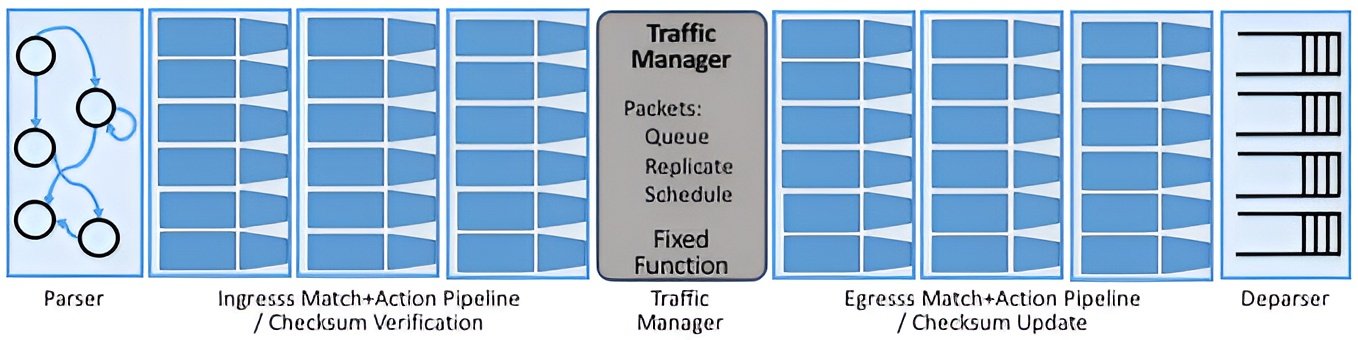
\includegraphics[width=0.8\textwidth]{archivos/img/teoria/softswitch.jpg}
    \caption{Arquitectura genérica de un \textit{softswitch} \gls{sdn} \cite{softswitches1}}
    \label{fig:softswitch}
\end{figure}

Según se puede apreciar en la figura \ref{fig:softswitch}, la arquitectura genérica de un \textit{softswitch} se puede resumir en los siguientes bloques. El primero de todos tiene que ser un parser, que vaya inspeccionando los paquetes entrantes a la pipeline de procesamiento del switch para identificar que tipo es. Una vez se ha identificado el paquete que se va a procesar, el siguiente bloque son las tablas de \textit{match-action}, las cuales tienen una interfaz de comunicación con el controlador \gls{sdn} para establecer criterios y campos de \textit{match}, y en caso de haber un \textit{match}, definir una serie de acciones para llevar a cabo. En función del \textit{softswitch}, la verificación de \textit{checksum}\footnote{Suma de comprobación, campo para comprobar la integridad del paquete de datos} se puede llevar a cabo en el parser o en la etapa de las tablas de \textit{match-action}. El siguiente bloque que nos podemos encontrar en un \textit{softswitch} es el conocido como gestor de tráfico, que variará en función de la implementación, pero nos proveerá de gestión de colas, \gls{qos}, duplicado de paquetes, etc. La siguiente etapa ya es más opcional, que se suele denominar como \textit{egress match-action}, la cual se puede utilizar para definir algún tipo de lógica a la salida de los switches, aunque en la realidad se suele utilizar para actualizar los campos  de \texttt{TTL} y recalcular el \textit{checksum} dado que el paquete se habrá visto modificado. El último bloque es el deparser, el cual se encarga de ensamblar de nuevo el paquete y prepararlo para sacarlo por el puerto de salida del switch.

\subsection{OvS}
\label{subsec:OVS}

\gls{ovs}, es uno de los \textit{softswitches} de referencia en el mundo de las redes, ampliamente utilizado tanto en la industria como en la academia. El switch está ofrecido como un proyecto opensource y respaldado por la Linux Foundation.  Es uno de los software switches más utilizados y ampliamente adoptados en entornos \gls{sdn} debido a su flexibilidad y funcionalidades avanzadas, aunque si tiene que destacar por algo, es por su gran rendimiento al trabajar a nivel de Kernel siendo idóneo para entornos de producción \cite{ovs1}. El \gls{ovs} actúa como un switch virtual, proporcionando capacidades de conmutación y reenvío para máquinas virtuales y contenedores en entornos de virtualización. Puede ejecutarse en hipervisores populares, como KVM (Kernel-based Virtual Machine), Xen y VMware, y también puede ser implementado como un switch independiente en instancias o servidores en modo standalone. Las características clave de Open vSwitch incluyen:

\begin{itemize}
    \item Agente \gls{sdn}: el switch ofrece una interfaz que permite que sea controlado mediante un controlador \gls{sdn}, como OpenDaylight o ONOS. Esto permite una gestión centralizada y un control más granular de la red, así como la implementación de políticas de red definidas por software.
    \item Funcionalidades avanzadas de alto rendimiento: \gls{ovs} ofrece una amplia gama de funcionalidades, como fast-forwarding al trabajar con frameworks como \gls{xdp}, DPDK o \gls{ebpf}. Estas características permiten una gestión eficiente de la red, y entorno de altas prestaciones ofreciendo un alto rendimiento perfecto para despliegues de producción.
    \item Integración con tecnologías de virtualización: \gls{ovs} se integra estrechamente con tecnologías de virtualización como OpenStack y Docker. Puede proporcionar conectividad de red entre máquinas virtuales, contenedores y hosts físicos, facilitando la migración y la gestión de recursos en entornos virtualizados.
    \item Extensibilidad y soporte para estándares: El \gls{ovs} es altamente extensible y se puede ampliar mediante la integración de módulos y complementos personalizados. Por ejemplo, para la integración del lenguaje de \gls{p4} se está haciendo de forma paulatina mediante módulos. Además, cumple con los estándares de la industria, como el protocolo OpenFlow, para garantizar la interoperabilidad con otros componentes \gls{sdn}.
\end{itemize}

Si nos fijamos en la figura \ref{fig:ovs}, podemos apreciar los componentes principales de la arquitectura del \gls{ovs}. Como se puede apreciar en la figura hay dos partes claramente diferenciadas en el \textit{softswitch}, una de espacio de usuario y otra parte de espacio de Kernel. Esta última es la que proveerá al \gls{ovs} de un alto rendimiento en comparación con otros software switches.  Los componentes principales del \gls{ovs} se pueden resumir en los siguientes puntos \cite{ovs1}.

\begin{itemize}
    \item \texttt{ovs-vswitchd}, es un \textit{daemon} que corre en espacio de usuario que implementa el switch, este proceso corre de forma conjunta con un módulo que corre en espacio de kernel, los cuales se comunican por netlink\footnote{\url{https://man7.org/linux/man-pages/man7/netlink.7.html}} para establecer la política de gestión de flujos.
    \item \texttt{ovsdb-server}, es un servidor de base de datos ligera, a la cual el proceso de espacio de usuario \texttt{ovs-vswitchd} le hace queries para obtener su configuración.
    \item \texttt{ovs-dpctl}, es una herramienta de gestión del módulo del kernel que implementa el datapath. El nombre de la herramienta hereda del nombre puesto a la herramienta original \texttt{dpctl}, la cual fue propuesta por Stanford en 2009\footnote{\url{https://github.com/mininet/openflow/blob/master/utilities/dpctl.c}}, y es un acrónimo de \textit{\textbf{d}ata\textbf{p}ath-\textbf{c}on\textbf{t}ro\textbf{l}}.
    \item \texttt{ovs-vsctl}, es uan utilidad para gestionar la configuración del proceso de espacio de usuario \texttt{ovs-vswitchd}.
    \item \texttt{ovs-appctl}, es una herramienta para mandar comandos a los \textit{daemon}s \gls{ovs}.
    \item \texttt{ovs-ofctl}, es una herramienta con la cual podemos mandar comandos y controlar vía OpenFlow el funcionamiento de switch.
    \item \texttt{ovs-testcontroller}, es un controlador experimental que implementan para testear la recepción y manejo de mensajes OpenFLow.
\end{itemize}

% fig
\begin{figure}[ht]
    \centering
    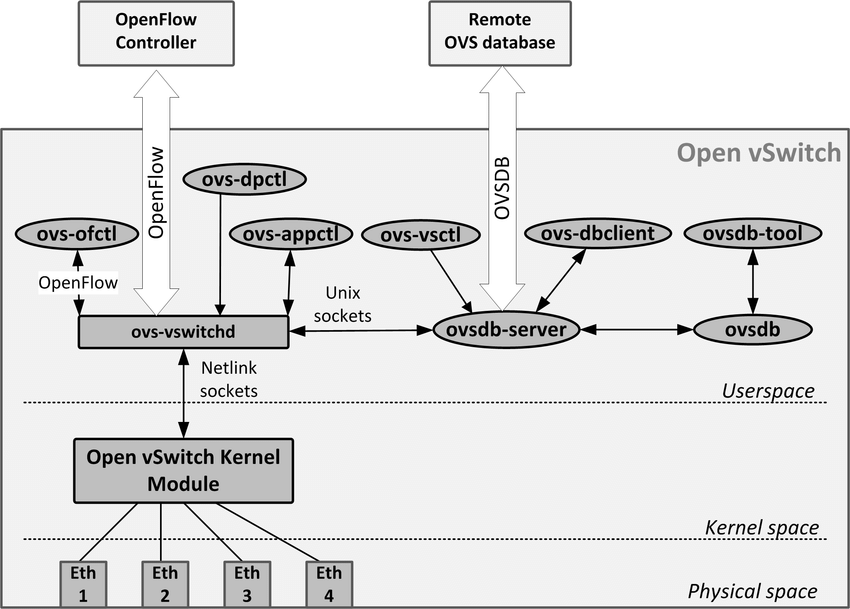
\includegraphics[width=0.7\textwidth]{archivos/img/teoria/ovs.png}
    \caption{Arquitectura del \glsentryshort{ovs} \cite{mendiola2016survey}}
    \label{fig:ovs}
\end{figure}

En resumen, el \gls{ovs} es un software switch \gls{sdn} ampliamente utilizado que proporciona capacidades avanzadas de conmutación y enrutamiento para entornos de virtualización. Su flexibilidad, funcionalidades avanzadas, rendimiento y compatibilidad con estándares lo convierten en una opción popular para implementaciones \gls{sdn} en diversos entornos, desde centros de datos hasta infraestructuras de proveedores de servicios.


\subsection{BOFUSS}
\label{subsec:BOFUSS}